%%%%%%%%%%%%%%%%%%%%%%%%%%%%%%%%%%%%%%%%%
% a0poster Portrait Poster
% LaTeX Template
% Version 1.0 (22/06/13)
%
% The a0poster class was created by:
% Gerlinde Kettl and Matthias Weiser (tex@kettl.de)
% 
% This template has been downloaded from:
% http://www.LaTeXTemplates.com
%
% License:
% CC BY-NC-SA 3.0 (http://creativecommons.org/licenses/by-nc-sa/3.0/)
%
%%%%%%%%%%%%%%%%%%%%%%%%%%%%%%%%%%%%%%%%%

%----------------------------------------------------------------------------------------
%	PACKAGES AND OTHER DOCUMENT CONFIGURATIONS
%----------------------------------------------------------------------------------------

\documentclass[a0,landscape]{a0poster}

\usepackage{multicol} % This is so we can have multiple columns of text side-by-side
\columnsep=50pt % This is the amount of white space between the columns in the poster
\columnseprule=3pt % This is the thickness of the black line between the columns in the poster

\usepackage[svgnames]{xcolor} % Specify colors by their 'svgnames', for a full list of all colors available see here: http://www.latextemplates.com/svgnames-colors

\usepackage{times} % Use the times font
%\usepackage{palatino} % Uncomment to use the Palatino font

\usepackage{graphicx} % Required for including images
\usepackage{booktabs} % Top and bottom rules for table
\usepackage[font=small,labelfont=bf]{caption} % Required for specifying captions to tables and figures
\usepackage{amsfonts, amsmath, amsthm, amssymb} % For math fonts, symbols and environments
\usepackage{wrapfig} % Allows wrapping text around tables and figures
\usepackage{algorithm} 
\usepackage{algorithmic}

\begin{document}

%----------------------------------------------------------------------------------------
%	POSTER HEADER 
%----------------------------------------------------------------------------------------

% The header is divided into two boxes:
% The first is 75% wide and houses the title, subtitle, names, university/organization and contact information
% The second is 25% wide and houses a logo for your university/organization or a photo of you
% The widths of these boxes can be easily edited to accommodate your content as you see fit

\begin{minipage}[b]{0.75\linewidth}
\veryHuge \color{NavyBlue} \textbf{VHASH: Spatial DHT based on Voronoi Tessellation} \color{Black}\\ % Title
\huge \textbf{Brendan Benshoof, Andrew Rosen, Anu Bourgeois \& Robert Harrison}\\[0.5cm] % Author(s)
\huge Georgia State Univerity Computer Science\\[0.4cm] % University/organization
\Large \texttt{bbenshoof@cs.gsu.edu}\\
\end{minipage}
%
\begin{minipage}[b]{0.25\linewidth}

\includegraphics[width=20cm]{logo.png}\\
\end{minipage}

\vspace{1cm} % A bit of extra whitespace between the header and poster content

%----------------------------------------------------------------------------------------

\begin{multicols}{5} % This is how many columns your poster will be broken into, a portrait poster is generally split into 2 columns

%----------------------------------------------------------------------------------------
%	ABSTRACT
%----------------------------------------------------------------------------------------

\color{Navy} % Navy color for the abstract

\begin{abstract}
%1. State the problem
Distributed Hash Tables are used as a tool to generate overlay networks for P2P networks. Current DHT techniques are not deisgned to take the nature of the unerlying network into acount when organizing the overlay network. Current DHT networks assign nodes locations in a ring or tree, limiting the ability of these networks to be more efficent.
%2. Say why it’s an interesting problem
A DHT technique that allows for efficent construction of an overlay network that takes into account the real underlying network would allow for higher proformance and faster P2P networks.
%3. Say what your solution achieves
We present VHASH as a spactial DHT based on approximate Delunay Triangulation to integrate distance information between nodes into overlay network topology.
%4. Say what follows from your solution
VHASH allows for the creation of P2P s with faster record lookup time, storage, and maintence with a geographically diverse set of nodes.

\end{abstract}

%----------------------------------------------------------------------------------------
%	INTRODUCTION
%----------------------------------------------------------------------------------------

\color{SaddleBrown} % SaddleBrown color for the introduction

\section{Introduction}
A Distributed Hash Table is used provide an overlay network for many P2P applications. State of the art DHT techniques are built on tree or log-ring structures to ensure that the routing distance is $O(lg(n))$ hops between nodes. This topologies, while sufficent in reasonably local networks, do not take into account the lengths of given hops. Current DHT techniques assume that every hop has similar latency and throuhput. For a global network, a more intellegent means of generating a dynamic overlay network with efficent routing, storage, and backups is needed for future P2P applications. We present VHASH as a DHT designed to take inter-node latency information into account when generating an overlay for massive scale use.

\color{DarkSlateGray} % DarkSlateGray color for the rest of the content

\section{VHash}
VHash was created to allow for spacial representations to be mapped to hash locations, a feature lacking in many current distributed hash tables.  In particular, we aimed to construct a mechanism for creating a more efficient global scale DHT built on a minimal latency overlay. Rather than focus on minimizing the amount of hops required to travel from point to point we wish to minimize the time required for a message to reach its recipient. VHash actually has a worse worst case hop distance ($O(\sqrt[d]{n})$) than other comparable distributed hash tables ($O(lg(n))$). However, VHash can route messages as quickly as possible rather than traveling over a grand tour that an overlay network may describe in the real world.

The naive method of doing so is to assign coordinates to servers based on the geographic location of nodes. More complex approaches would approximate a minimum latency space based on inter-node latency. VHash can be considered  a generalized extension of VoroNet \cite{voronet}.  %Why is Voronet not okay and why is VHash

%The intent is that meaning can be ascribed to locations in the DHT and facilitate more efficent function. 
%Specifically in this example we seek to build a minimal latency overlay network for the DHT so a global scale DHT is viable and efficent. 











\subsection{Toroidal Distance Equation}

Given two vector locations $\vec{a}$ and $\vec{b}$ on a  $d$ dimensional unit toroidal hypercube:
\[ distance = \sqrt[|d|]{\sum\limits_{i\in d} (\min(|\vec{a}_i-\vec{b}_i|,1.0-|\vec{a}_i-\vec{b}_i|))^2}\]

\subsection{Mechanism}
VHash maps nodes to a $d$ dimension toroidal unit space overlay. This is essentially a hypercube with wrapping edges. The toroidal property makes visualization difficult but allows for a space without a sparse edge, as all nodes can translate the space such that they are at the center of the space.  In effect, each node views itself at the center of the graph.

VHash nodes are responsible for the address space defined by their Voronoi region. This region is defined by a list of peer nodes maintained by the node. A minimum list of peers is maintained such that the node's Voronoi region is well defined. The links connecting the node to its peers correspond to the links of a Delaunay Triangulation.  One such possible network is shown on Figure \ref{churninit}.


\begin{figure}[H]
    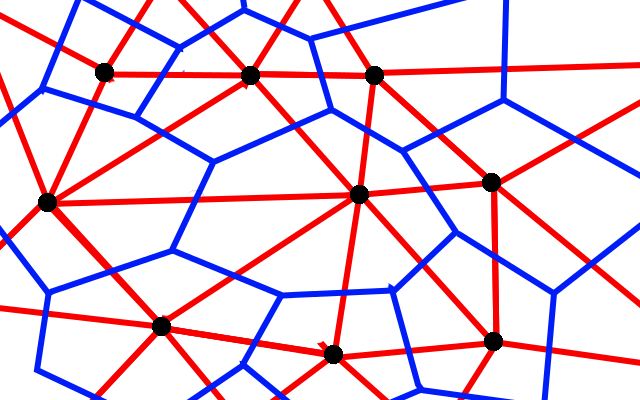
\includegraphics[width=\linewidth]{voronoi-churn2}
    \caption{The starting network topology.  The blue lines demark the Voronoi edges, while the red lines connecting the nodes correspond to the Delaunay Triangulation edges and one-hop connections.}
    \label{churninit}
\end{figure}

\subsection{Relation to Voronoi Diagrams and Delaunay Triangulation}

VHash does not strictly solve Voronoi diagrams \cite{voronoi}, as the toroidal nature of the space preclude the traditional means of solving for Voronoi regions. However, VHash's peer management approximates a topology with similar properties. 
%Rather than attempt to calculate the Voronoi region of each node, it simply filters locations, assigning responsibility to the nearest node. 
An online algorithm (Algorithm \ref{peer} maintains the set of peers defining the node's voronoi region. The set of peers required to define a node's Voronoi Region corresponds to a solution to the dual Delaunay Triangulation.



\begin{algorithm}[H]
\caption{VHash Greedy Peer Selection}
\label{peer}
\begin{algorithmic}[1]  % the number is how many 
	\STATE $Candiates$ is the set of candidate peers
    \STATE $Peers$ is the set of this node's peers
    \STATE $Canidates$ is sorted by each node's closeness to this node
    \STATE The closest member of $Canidates$ is popped and added to $Peers$
    \FORALL{$n$ in $Canidates$}
    	\STATE $c$ is the midpoint between this node and $n$
        \IF{Any node in $Peers$ is closer to $c$ than this node}
        	\STATE reject $n$ as a peer
        \ELSE
        	\STATE Add $n$ to $Peers$
        \ENDIF
    \ENDFOR
\end{algorithmic}
\end{algorithm}


\subsection{Messages}
Maintenance and joining are handled by a simple periodic mechanism. A notification message consisting of a node's information and active peers is the only maintenance message. All messages have a destination hash location which is used to route them to the proper server. This destination can be the hash location of a particular node or the location of a desired record or service.  The message is received by the node responsible for the location. Services running on the DHT define their own message contents, such as commands to store and retrieve data.

\subsection{Message Routing}
When routing a message to an arbitrary location, a node calculates who's voronoi region the message's destination is in amongst the itself and its peers. If the destination falls within its own region, then it is responsible and handles the message accordingly. Otherwise, the node forwards the message to the closest peer to the destination location. This process describes a pre-computed and cached A* routing  algorithm \cite{astar} . 

\subsection{Joining and Maintenance}
Joining the network is a straightforward process. A new node first learns the location of at least one member of the network to join. The joining node then choses a location in the hash space either at random or based on a problem formulation (for example, based on geographic location or latency information).

After choosing a location, the joining node sends a "join" message to its own location via the known node.
The message is forwarded to the current owner of that location who can be considered the "parent" node.
The parent node immediately replies with a maintenance message containing its full peer list. This message is sent to the joining node, who then uses this to begin defining the space it is responsible for. 

The joining node's initial peers are a subset of the parent and the parent's peers. The parent adds the new node to its own peer list and removes all his peers occluded by the new node.  Then regular maintenance propagates the new node's information and repairs the overlay topology.  This process is described by Algorithm \ref{join}.

\begin{algorithm}[H]
\caption{Vhash Join}
\label{join}
\begin{algorithmic}[1]  % the number is how many 
\STATE new node $N$ wishes to join and has location $L$
\STATE $N$ knows node $x$ to be a member of the network
\STATE $N$ sends a request to join, addressed to $L$ via $x$
\STATE node $Parent$ is responsible for location $L$ and receives the join message
\STATE $Parent$ sends to $N$ its own location and list of peers
\STATE $Parent$ integrates $N$ into its peer set
\STATE $N$ builds its peer list from $N$ and its peers
\STATE regular maintenance updates other peers
\end{algorithmic}
\end{algorithm}


Each node in the network performs maintenance periodically by a maintenance message to its peers. The maintenance message consists of the node's information and the information on that node's peer list. When a maintenance message is received, the receiving node considers the listed nodes as candidates for its own peer list and removes any occluded nodes (Algorithm \ref{peer}). 

When messages sent to a peer fail, it is assumed the peer has left the network. The leaving peer is removed from the peer list and candidates from the set of 2-hop peers provided by other peers move in to replace it.   

There is no function for a "polite" exit from the network. VHash  assumes nodes will fail and the difference between an intended failure and unintended failure is unnecessary. The only issue this causes is that node software should be designed to fail totally when issues arise rather then attempt to fulfill only part of its responsibilities.  



\subsection{Data Storage and Backups}
The primary goal of a DHT is to provide a distributed storage medium. We extend this idea to distribute work and information among nodes using the same paradigm. Resources in the network, be it raw data or assigned tasks, are assigned hash locations. The node responsible for a given hash location is responsible for the maintenance of that resource. When a node fails, its peers take responsibility of its space. Thus it is important to provide peers with frequent backups of a node's assigned resources.  That way, when a node fails, its peers can immediately assume its responsibilities.

When a resource is to be stored on the network, it is assigned a hash location. The hash locations assigned could be random, a hash of an identifier, or have specific meaning for an embedding problem. The node responsible for that resource's hash location stores the resource.

A resource is accessed by contacting the node responsible for the resource.  However, the requester generally has no idea which node is responsible for any particular resource.  The data request messsage is addressed to the location corresponding to the resource, rather than the node responsible for that location.  The message is forwarded over the overlay network, each hop bringing the node closer until it reaches the responsible node, who sends the resource or an error if the resource does not exist.

Some options are immediately apparent for dealing with wasted storage space. A system that is primarily read driven can record the time of the last read or a frequency of reads such that resources that are not read often enough are deleted after a certain period of time. If a system is write driven, allow the resource to be assigned a time to live, which can be updated as needed.

A node periodically sends a message containing backups of the resources for which it became newly responsible for to each of its peers. To minimize bandwidth and time wasted by backups, the node should only send the records changed since last backup.

\bibliographystyle{ieeetr}
\bibliography{P3DNS}----------

\end{multicols}
\end{document}